% ============================================================================
%  第 1 章  $A_\infty$-代数  （原书 pp.5–9，PDF pp.8–12）
% ============================================================================
\section{$A_\infty$-代数}\label{ch:01}

\takeaway{%
  核心图像：环路空间的拼接只在同伦意义下结合；结合的失效由一族高阶同伦 $m_n$ 逐级补偿，
  其组合模式正是结合面体 $K_n$。\\
  数学工具：分次向量空间与 Koszul 符号法则、上链复形、结合面体、$A_\infty$-代数与
  $A_\infty$-模的方程。\\
  主要结论：$A_\infty$-代数在上同调层面退化为分次结合代数；$A_\infty$-模及其态射构成范畴
  $\mathcal C_\infty(\mathcal A)$，为第一部分的一般理论提供原型。%
}

\subsection{非结合性示例：$A_\infty$-空间}\label{sec:1.1}

让我们从一个拓扑例子开始对 $A_\infty$-代数的研究，它最清楚地揭示了非结合性这一概念。
设 $(X,x_0)$ 为带基点的拓扑空间，
$\Omega X:=\{f:[0,1]\to X\mid f\ \text{连续},\ f(0)=f(1)=x_0\}$
为 $X$ 中以 $x_0$ 为基点的环路空间。通过拼接环路，我们可以定义复合映射
$m_2:\Omega X\times\Omega X\to\Omega X$，$(f_1,f_2)\mapsto(f_1*f_2)$，其中
\[
  (f_1*f_2)(t):=
  \begin{cases}
    f_1(2t) & \text{若 } 0\le t\le 1/2,\\
    f_2(2t-1) & \text{若 } 1/2\le t\le 1 .
  \end{cases}
\]
于是所得环路"把一半时间"花在 $f_1$ 上，另一半花在 $f_2$ 上。

显然 $m_2$ 不结合：对第三个环路 $f_3\in\Omega X$，有
$m_2(m_2(f_1,f_2),f_3)\neq m_2(f_1,m_2(f_2,f_3))$——在第一种拼接中，沿 $f_1$ 只走了
"四分之一的时间"，而在第二种中走了一半。

不过，我们可以借助同伦 $m_3:[0,1]\times(\Omega X)^3\to\Omega X$ 改变时间分配，把拼接
$(f_1*f_2)*f_3$ 连续形变为 $f_1*(f_2*f_3)$。同一个 $m_3$ 还可用来在四个环路的五种可能
拼接之间移动：
$(f_1*(f_2*f_3))*f_4$、$((f_1*f_2)*f_3)*f_4$、$(f_1*f_2)*(f_3*f_4)$、
$f_1*(f_2*(f_3*f_4))$ 以及 $f_1*((f_2*f_3)*f_4)$。把这些构型示意地画成某个图的顶点，
让图的边表示 $m_3$ 所走的路径，最终得到的是一个五边形的边界。记之为 $K_4$。

依此类推，对一般的 $n>3$，通过归纳地定义同伦
$m_n:K_n\times(\Omega X)^n\to\Omega X$，可以把上述构造推广到一般的 $(n-2)$ 维多胞体
$K_n$（约定 $K_2:=\{*\}$，$K_3:=[0,1]$；见图 1）。

\begin{figure}[htbp]
  \centering
  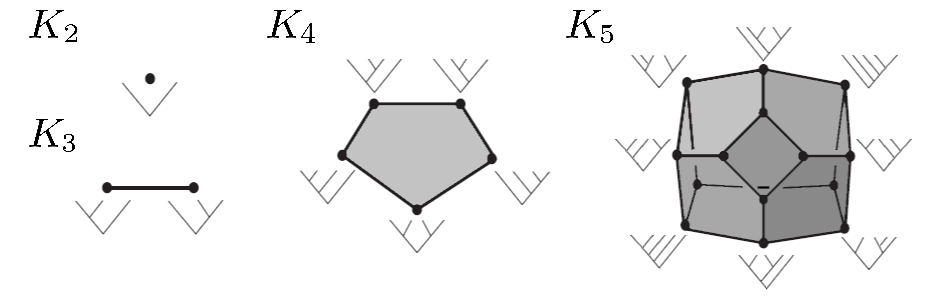
\includegraphics[width=0.72\linewidth]{fig01.png}
  \caption{前四个结合面体 $K_2,K_3,K_4,K_5$。顶点处的每一种拼接都可用一棵二叉树表示：
    例如 $K_2$ 只含一个点 $(f_1*f_2)\in\Omega X$，其二叉树平凡；$K_3$ 有两个顶点，分别对应
    $((f_1*f_2)*f_3)$ 与 $(f_1*(f_2*f_3))$；构成 $K_4$ 的各种拼接已在正文列出。另一方面，
    更高维的胞腔参数化分叉更多的树：例如 $K_3$ 的 1-胞腔由一棵三叉树标记，编码
    $f_1*f_2*f_3$。[来源：\texttt{http://pseudomonad.blogspot.com/2010/08/m-theory-lesson-345.html}]
    \hfill（原书 p.5）}
  \label{fig:01}
\end{figure}

这些 $K_n$ 称为\textbf{结合面体}（associahedra），由 Stasheff 在 \cite{Sta63} 中首次构造。
他把它们纳入 $A_\infty$-空间的定义：$A_\infty$-空间是带有相容映射族
$m_n:K_n\times Y^n\to Y$（$n\ge 2$）的拓扑空间 $Y$。如上所见，环路空间 $\Omega X$ 正是
$A_\infty$-空间的原型。此外，对任何这样的 $Y$，奇异上链复形 $C^\bullet(Y)$ 给出我们所遇到的
第一个 $A_\infty$-代数。下面说明其缘由。

\subsection{$A_\infty$-代数与态射}\label{sec:1.2}

全文中我们总在一个固定的基域 $\mathbb K$ 上工作，并假定分次取在 $\mathbb Z$ 上，除非另有
说明。我们先回顾分次向量空间与复形的基本内容（参看 \cite{Kel06} 第 2.1 节）。

\begin{Def}\label{def:1.1}
设 $V$ 为 $\mathbb Z$-分次 $\mathbb K$-向量空间，即形如 $V=\bigoplus_{p\in\mathbb Z}V^p$。
对 $n\in\mathbb Z$，其 \textbf{$n$ 次平移} $V[n]$ 是把所有指标向下移动 $n$ 次所得的分次向量空间，
即 $(V[n])^p=V^{p+n}$ 对一切 $p\in\mathbb Z$ 成立。记 $SV:=V[1]$，称之为 $V$ 的
\textbf{悬挂}（suspension）。

给定另一个分次向量空间 $V'$，分次向量空间之间的态射 $f:V\to V'[d]$ 是次数为
$d=|f|\in\mathbb Z$ 的齐次分次 $\mathbb K$-线性映射（于是次数为 $p=|v|$ 的齐次元素
$v\in V$ 被映为次数为 $p+d$ 的齐次元素 $f(v)\in V'$；为方便起见，我们常常省略态射的次数信息）。

分次向量空间及其态射构成范畴 $\mathsf{GradVect}$。
\end{Def}

考虑分次向量空间态射 $f:V\to V'$ 与 $g:W\to W'$ 的张量积
$f\otimes g:V\otimes W\to V'\otimes W'$ 时，结果服从 \textbf{Koszul 符号法则}：
\[
  (f\otimes g)(v\otimes w)=(-1)^{|g||v|}f(v)\otimes g(w),
\]
对一切齐次元素 $v\in V$，$w\in W$ 成立。

\begin{Def}\label{def:1.2}
若分次向量空间 $V$ 带有一个微分 $d_V:V\to V[1]$，即一个满足 $d_V\circ d_V=0$ 的 1 次齐次
态射，则称之为一个\textbf{（上链）复形}。我们定义 $d_{SV}:=-d_V$，并对分次向量空间态射
$f:V\to V'$ 定义
\[
  d(f):=d_{V'}\circ f-(-1)^{|f|}f\circ d_V .
\]
后者成为复形态射（上链映射）当且仅当 $d(f)=0$。

复形及其态射构成范畴 $\mathsf{Ch}$。因此我们可以研究它的上同调对应物 $H(\mathsf{Ch})$：
其对象是分次向量空间 $H(V)=\bigoplus_{p\in\mathbb Z}H^p(V)$，态射是诱导出的分次态射
（确实，作为范畴有 $H(\mathsf{Ch})\simeq\mathsf{GradVect}$）。
\end{Def}

最后回顾：复形态射 $f$ 与 $f'$ 同伦，当且仅当存在分次向量空间态射 $h$ 使得
$f-f'=d(h)$。同调代数学告诉我们，此时两者在上同调中诱导的映射相同：
$H^p(f)=H^p(f')$ 对一切 $p\in\mathbb Z$ 成立。

下面我们定义 $A_\infty$-代数，它也称为\textbf{强同伦结合代数}（strongly homotopy
associative algebra），其缘由将在下面的注 \ref{rem:1.5} 中明了。主要参考文献是
\cite{Kel01} 第 3–4 节。

\begin{Def}\label{def:1.3}
域 $\mathbb K$ 上的 \textbf{$A_\infty$-代数}是一个 $\mathbb Z$-分次 $\mathbb K$-向量空间
$A=\bigoplus_{p\in\mathbb Z}A^p$，带有分次态射 $m_n:A^{\otimes n}\to A[2-n]$（$n\ge 1$），
使得对一切 $n\ge 1$，作为 $A^{\otimes n}\to A$ 的映射成立方程
\begin{equation}\label{eq:1.1}
  \sum_{r+s+t=n}(-1)^{r+st}m_{r+1+t}
  \bigl(\mathrm{id}_A^{\otimes r}\otimes m_s\otimes\mathrm{id}_A^{\otimes t}\bigr)=0 .
\end{equation}
若 $A$ 带有某个 $1_A\in A^0$，使得 $m_1(1_A)=0$，
$m_2(1_A,a)=a=m_2(a,1_A)$ 对一切 $a\in A$ 成立，且当 $i>2$ 时
$m_i(\dots,1_A,\dots)=0$，则称 $A$ \textbf{严格幺的}（strictly unital）。
（若 $1_A$ 存在则唯一；称之为\textbf{严格单位元}。）

$A$ 的 \textbf{$A_\infty$-子代数} $B$ 是一个分次子空间，使得所有态射 $m_n$ 都限制到 $B$ 上。
\end{Def}

% [Tutor Note: 【易错】式 \eqref{eq:1.1} 的符号指数是 $r+st$，不是 $r+s+t$ 或 $rs+t$。它来自
% 把 $m_s$ 搬过前 $r$ 个因子的 Koszul 符号：$(-1)^{s\cdot 1\cdot r}$（每个 $m_s$ 的次数为
% $2-s$，故实际指数为 $r(2-s)+st$ 的化简结果，见 Keller 书中的推导）。逐项核对时务必先固定
% $r,s,t$ 再数 $m_s$ 与 $m_{r+1+t}$ 的相对位置。]

这里我们不必过分纠结式 \eqref{eq:1.1} 中出现的符号：具体的输入会按定义 \ref{def:1.1} 的
Koszul 法则对它作相应修改。在讨论 $A_\infty$-范畴时我们会更精确，那里所有公式都以这种形式
给出。

\begin{Rem}\label{rem:1.4}
若希望让定义 \ref{def:1.3} 中每个态射 $m_n$ 的次数与 $n$ 无关，有一种借助悬挂的典范做法：
通过要求下图交换，在诸 $m_n$ 与分次映射 $b_n:(SA)^{\otimes n}\to SA$ 之间建立一一对应：
\[
  \begin{tikzcd}
    A^{\otimes n} \arrow[r,"m_n"] \arrow[d,"s^{\otimes n}"'] & A \arrow[d,"s"] \\
    (SA)^{\otimes n} \arrow[r,"b_n"'] & SA
  \end{tikzcd}
\]
对一切 $n\ge 1$ 成立。这里 $s:A\to SA$，$a\in A^p\mapsto a\in(SA)^{p-1}$，次数为 $-1$，
于是每个 $b_n$ 满足 $|b_n|=-(-1)\cdot n+(2-n)+(-1)=1$。特别地，$b_1=-m_1$，且
$b_2(a_1,a_2)=(-1)^{|a_1|}m_2(a_1,a_2)$。可以证明：诸 $m_n$ 在 $A$ 上给出 $A_\infty$-代数
结构，当且仅当对一切 $n\ge 1$，
\[
  \sum_{r+s+t=n}b_{r+1+t}
  \bigl(\mathrm{id}_A^{\otimes r}\otimes b_s\otimes\mathrm{id}_A^{\otimes t}\bigr)=0 ,
\]
其中可以注意到，式 \eqref{eq:1.1} 中的符号已经消失。

具体操作中我们几乎从不真正使用悬挂，但在拼合各种符号约定时必须把它们考虑在内。
\end{Rem}

% [Tutor Note: 【含糊】注 \ref{rem:1.4} 中 "可以证明"（原文 one can prove）省略了证明：它等价于
% 同调微扰引理（HPT）在一维情形下的表述——把 $m_n$ 用 $s^{\otimes n}$ 共轭并消去 $\pm1$ 因子，
% 或用 $b_n=s\circ m_n\circ(s^{\otimes n})^{-1}$ 直接验证方程逐项相消。$|b_n|$ 的计算中
% "$-(-1)\cdot n$" 一项是 $(s^{\otimes n})^{-1}$ 的次数 $+n$（因为 $|s|=-1$），作者写成
% $(-1)\cdot n$ 再取负，易误读数。参见 Keller \cite{Kel01} 第 3 节。]

\begin{Rem}\label{rem:1.5}
方程组 \eqref{eq:1.1} 给出以下推论：
\begin{itemize}[leftmargin=2em]
  \item $m_1m_1=0$，于是 $(A,m_1)$ 是上链复形（从而按定义 $(SA,-m_1)$ 也是）。
  \item $m_1m_2=m_2(m_1\otimes\mathrm{id}_A+\mathrm{id}_A\otimes m_1)$ 表明微分 $m_1$ 是乘法%
  \footnote{我们称之为"乘法"，是因为在 $p\neq 0$ 时 $A^p=0$ 的特殊情形下，$A=A^0$ 只有
  $m_2$ 这一个非零映射，其次数为 $0$，因而可看作普通结合代数 $A$ 的乘法。}
  $m_2$ 的导子（即按分次 Leibniz 法则相容——正如所预期的那样）。由于
  $(m_1\otimes\mathrm{id}_A+\mathrm{id}_A\otimes m_1)$ 是 $A^{\otimes 2}$ 的微分，$m_2$ 是
  复形态射。
  \item $m_2(\mathrm{id}_A\otimes m_2-m_2\otimes\mathrm{id}_A)
  =m_1m_3+m_3(m_1\otimes\mathrm{id}_A\otimes\mathrm{id}_A+\mathrm{id}_A\otimes m_1\otimes
  \mathrm{id}_A+\mathrm{id}_A\otimes\mathrm{id}_A\otimes m_1)=d(m_3)$ 告诉我们：$m_2$ 只在
  同伦意义下结合！（"强同伦结合"这一术语即由此而来。）因此相应的上同调 $H(A)$ 关于
  $H(m_2)$ 构成分次结合代数（若 $H(A)$ 有单位元，则它由 $A$ 的上同调单位元诱导）。
  \item 若对一切 $n>2$ 有 $m_n=0$，则 $(A,m_1,m_2)$ 成为结合微分分次代数；反之，任何这样
  的代数都可看作 $A_\infty$-代数的特例。
\end{itemize}
\end{Rem}

第二个要点揭示了 $A_\infty$-代数的本性：它是结合性只在上同调意义下成立（且可能没有单位元）
的代数。第三个要点则已预示了在上同调层面工作的优势，这是我们后续理论的一条指导原则。

\begin{Def}\label{def:1.6}
给定两个 $A_\infty$-代数 $A$ 与 $B$，其态射分别为 $m_n^A$ 与 $m_n^B$，则
\textbf{$A_\infty$-代数态射} $f:A\to B$ 是一族分次映射 $f_n:A^{\otimes n}\to B[1-n]$
（$n\ge 1$），满足方程
\begin{equation}\label{eq:1.2}
  \sum_{r+s+t=n}(-1)^{r+st}f_{r+1+t}
  \bigl(\mathrm{id}_A^{\otimes r}\otimes m_s^A\otimes\mathrm{id}_A^{\otimes t}\bigr)
  =\sum_{\substack{1\le r\le n\\ s_1+\cdots+s_r=n}}(-1)^u\,
  m_r^B(f_{s_1}\otimes\cdots\otimes f_{s_r})
\end{equation}
对一切 $n\ge 1$ 成立，其中 $u:=\sum_{i=1}^{r-1}(r-i)(s_i-1)$。

与第二个 $A_\infty$-代数态射 $g:B\to C$ 的复合由下列分次映射族给出：
\[
  (g\circ f)_n:=\sum_{\substack{1\le r\le n\\ s_1+\cdots+s_r=n}}(-1)^u\,
  g_r\circ(f_{s_1}\otimes\cdots\otimes f_{s_r})
\]
（把它们代入式 \eqref{eq:1.2} 即可看出 $g\circ f:A\to C$ 确实是 $A_\infty$-代数态射）。

当 $A=B$ 时容易看出：取 $f_1:=\mathrm{id}_A$ 而其余 $f_n:=0$ 的 $f$ 对应于 $A$ 上的恒等态射。
\end{Def}

% [Tutor Note: 【易错】式 \eqref{eq:1.2} 右端的符号指数 $u=\sum_{i=1}^{r-1}(r-i)(s_i-1)$
% 极易抄错：每一项是 $(r-i)(s_i-1)$，不是 $(r-i)(s_i)$，也不含 $f$ 自身的次数。它来自把
% $m_r^B$ 依次搬过 $f_{s_1},\dots,f_{s_i}$ 时累积的 Koszul 符号。验证 $n=2$ 的项
% $f_1m_2^A-m_2^B(f_1\otimes f_1)=d(f_2)$ 是符号是否抄对的试金石。]

特别地，式 \eqref{eq:1.2} 的前两个等式
$f_1m_1^A=m_1^Bf_1$ 与
$f_1m_2^A-m_2^B(f_1\otimes f_1)
=m_1^Bf_2+f_2(m_1^A\otimes\mathrm{id}_A+\mathrm{id}_A\otimes m_1^A)=d(f_2)$
告诉我们：$f_1$ 是复形态射，且只在与 $m_2$ 同伦的意义下与 $m_2$ 交换。同样，使用悬挂后
式 \eqref{eq:1.2} 中的符号即可省去（见注 \ref{rem:1.4}）。

最后我们给出几个稍后会在其 $A_\infty$-范畴形式中重现的定义。

\begin{Def}\label{def:1.7}
若 $A_\infty$-代数态射 $f:A\to B$ 的 $f_1$ 是拟同构，即它诱导出代数同构
$H(f_1):H(A)\to H(B)$，则称 $f$ 为\textbf{拟同构}。

严格幺 $A_\infty$-代数之间的态射 $f:(A,1_A)\to(B,1_B)$，若满足 $f_1(1_A)=1_B$ 且
$f_i(\dots,1_A,\dots)=0$（$i>1$），则称 $f$ 本身是\textbf{严格幺的}。
\end{Def}

\subsection{$A_\infty$-模与态射}\label{sec:1.3}

\begin{Def}\label{def:1.8}
设 $A$ 为 $A_\infty$-代数，其态射 $m_n^A$ 如定义 \ref{def:1.3} 所述。$A$ 上的
\textbf{$A_\infty$-模}是一个 $\mathbb Z$-分次 $\mathbb K$-向量空间
$M=\bigoplus_{p\in\mathbb Z}M^p$，带有映射 $m_n^M:M\otimes A^{\otimes n-1}\to M[2-n]$
（$n\ge 1$），它们满足与式 \eqref{eq:1.1} 类似的方程
\begin{equation}\label{eq:1.3}
  \begin{aligned}
    \sum_{r+s+t=n}(-1)^{r+st}m_{r+1+t}^M
    \bigl(\mathrm{id}_M\otimes\mathrm{id}_A^{\otimes r-1}\otimes m_s^A
    \otimes\mathrm{id}_A^{\otimes t}\bigr)&=0
    &&\text{若 } r>0,\\
    \sum_{s+t=n}(-1)^{st}m_{1+t}^M\bigl(m_s^M\otimes\mathrm{id}_A^{\otimes t}\bigr)&=0
    &&\text{若 } r=0.
  \end{aligned}
\end{equation}
\end{Def}

\begin{Def}\label{def:1.9}
设 $M$ 与 $N$ 为 $A_\infty$-代数 $A$ 上的 $A_\infty$-模，其态射分别为 $m_n^M$ 与 $m_n^N$。
\textbf{$A_\infty$-模态射} $f:M\to N$ 是一族分次映射
$f_n:M\otimes A^{\otimes n-1}\to N[1-n]$（$n\ge 1$），满足方程
\begin{equation}\label{eq:1.4}
  \sum_{r+s+t=n}(-1)^{r+st}f_{r+1+t}
  \bigl(\mathrm{id}_A^{\otimes r}\otimes m_s^M\otimes\mathrm{id}_A^{\otimes t}\bigr)
  =\sum_{s+t=n}(-1)^{(s+1)t}m_{1+t}^N\bigl(f_s\otimes\mathrm{id}_A^{\otimes t}\bigr)
\end{equation}
对一切 $n\ge 1$ 成立；其中必须像上一个定义那样区分 $r>0$ 与 $r=0$ 两种情形。

与第二个 $A_\infty$-模态射 $g:N\to P$ 的复合由下列分次映射族给出：
\[
  (g\circ f)_n:=\sum_{s+t=n}(-1)^{(s-1)t}f_{1+t}\circ\bigl(g_s\otimes
  \mathrm{id}_A^{\otimes t}\bigr)
\]
（可以证明它们满足方程 \eqref{eq:1.4}）。恒等态射与拟同构的定义与 $A_\infty$-代数情形相同。

$A_\infty$-模连同 $A_\infty$-模态射构成一个范畴，记作 $\mathcal C_\infty(\mathcal A)$。
\end{Def}

% [Tutor Note: 【易错】定义 \ref{def:1.9} 中 $r=0$ 的分支在式 \eqref{eq:1.4} 右端出现，
% 但左端求和仍写作 $r+s+t=n$；实际约定是：$r=0$ 时左端只剩 $s+t=n$ 的项且
% $m_s^M$ 直接作用在 $M$ 上。书写代码时若把两个分支合并，最常见错误是漏掉 $r=0$ 时
% $m_s^M$ 前少一个 $\mathrm{id}_A^{\otimes r}$ 因子。

现在我们已经初步领略了第一部分所处理的代数结构，接下来转向更一般的 $A_\infty$-范畴概念。
